%!TEX root = index.tex
\chapter{Desenvolvimento da biblioteca} % (fold)
\label{cha:desenvolvimento_da_biblioteca}

\section{Recursos acadêmicos} % (fold)
\label{sec:recursos_acad_micos}

Diversos recursos extra-curriculares foram de fundamental importância para o sucesso deste trabalho. Foram aplicados ensinamentos práticos de quatro cursos da plataforma online de \textit{e-learning} Coursera (\url{https://www.coursera.org/}), seja relacionados a teoria dos sistemas de recomendação, seja relacionados a configuração de máquinas virtuais dos servidores da Amazon Web Services.

O curso ``Redes: Amigos, Dinheiro e Bytes'' (Networks: Friends, Money, and Bytes -- \url{https://www.coursera.org/course/friendsmoneybytes}), teve papel importante na introdução a temas ligados à rede mundial de computadores. Mais especificadamente, a aula 4 aborda, de maneira simples mas repleta de exemplos, a temática de sugestão de itens através da pergunta ``Como o Netflix recomenda filmes?''. Essa aula ajudou-nos a compreender a teoria por trás do algoritmo de recomendação do Netflix detalhado na Referência \citeonline{lops2011content-chap5}.


Outro curso que influenciou diretamente o nosso Trabalho de Conclusão de Curso foi ``Computação para Análise de Dados'' (Computing for Data Analysis -- \url{https://www.coursera.org/course/compdata}). As quatro semanas de aula ensinaram a leitura de dados formatados em R, o tratamento de dados, a definição de métodos estatísticos, como por exemplo de regressão linear, a aplicação de cálculos vetorizados e a construção de gráficos e tabelas. 

Aliado a essas aulas, aprendemos também o paradigma funcional, amplamente utilizado em R, durante as sete semanas de ``Princípios de Programação Funcional em Scala'' (Functional Programming Principles in Scala -- \url{https://www.coursera.org/course/progfun}).

Por fim, o curso de doze semanas de duração ``Engenharia de Startup'' (Startup Engineering -- \url{https://www.coursera.org/course/startup}) nos ensinou a trabalhar com diversas ferramentas de software necessárias para a realização dos testes de desempenho dos algoritmos. Utilizamos máquinas virtuais, linha de comando Unix, editores de texto sem interface gráfica (tais como vi e Emacs). Além disso, o \textit{setup} de máquinas virtuais na Amazon Web Services também era abordada no curso, facilitando a configuração do ambiente de testes e a automatização desse processo. Visto que o serviço é cobrado por hora-máquina, desenvolvemos um \textit{script} de configuração em \texttt{bash}, que descarregava os pacotes necessários para a realização imediata dos testes, permitindo assim reduzir os custos da análise.   

\section{Ferramentas utilizadas} % (fold)
\label{sec:ferramentas_utilizadas}

A programação da biblioteca computacional se deu por meio do ambiente de desenvolvimento integrado RStudio versão 0.98.953 (\url{http://www.rstudio.com/}). Esse IDE inclui um console, um editor de texto e um corretor de sintaxe que suporta a execução de código direta, bem como ferramentas para traçar gráficos, histórico de comandos, depuração de erros e gerenciamento de espaço de trabalho. Além disso, o RStudio está disponível via licença de código aberto AGPLv3 (Affero General Public License version 3) para os principais sistemas operacionais (Windows, Mac e Linux).

\section{Métodos computacionais} % (fold)
\label{sec:m_todos_computacionais}

TODO falta escrever

\subsection{Algoritmo baseado na ponderação de atributos (FW)} % (fold)
\label{sub:algoritmo_baseado_na_pondera_o_de_atributos_fw_}
\subsection{Algoritmo baseado no perfil de usuários (UP)} % (fold)
\label{sub:algoritmo_baseado_no_perfil_de_usu_rios_up_}
\subsection{Algoritmo baseado na correlação usuário-item (UI)} % (fold)
\label{sub:algoritmo_baseado_na_correla_o_usu_rio_item_ui_}

% subsection algoritmo_baseado_na_correla_o_usu_rio_item_ui_ (end)

% subsection algoritmo_baseado_no_perfil_de_usu_rios_up_ (end)

% subsection algoritmo_baseado_na_pondera_o_de_atributos_fw_ (end)

\section{Ambiente de testes} % (fold)
\label{sec:ambiente_de_testes}

As etapas de configuração do ambiente de testes envolvem o cadastro na Amazon Web Services, a criação de uma máquina virtual e a instalação de todas as ferramentas necessárias na máquina.

Após o cadastro na AWS, deve-se seguir os seguintes passos para a criação de uma máquina virtual:


\begin{enumerate}
\item Login na plataforma (Figura \ref{fig:aws_servicos})
\item Acesso ao serviço de máquinas virtuais Elastic Compute Cloud ou EC2 (Figura \ref{fig:aws_ec2})
\item Escolha do tipo de configuração do software da máquina, como sistema operacional (Figura \ref{fig:aws_setup_ec2})
\item Escolha do tipo de máquina. No nosso caso, escolhemos uma máquina otimizada para memória RAM (Figura \ref{fig:aws_setup_ec2_maquina})
\item Criação da chave privada a ser utilizada para conexão com a máquina (Figura \ref{fig:aws_setup_keypair})
\item Criação da máquina e do DNS público. Esse é o endereço de conexão com a máquina (Figura \ref{fig:aws_setup_dns})
\end{enumerate}

\begin{figure}[htp]
    \begin{center}
    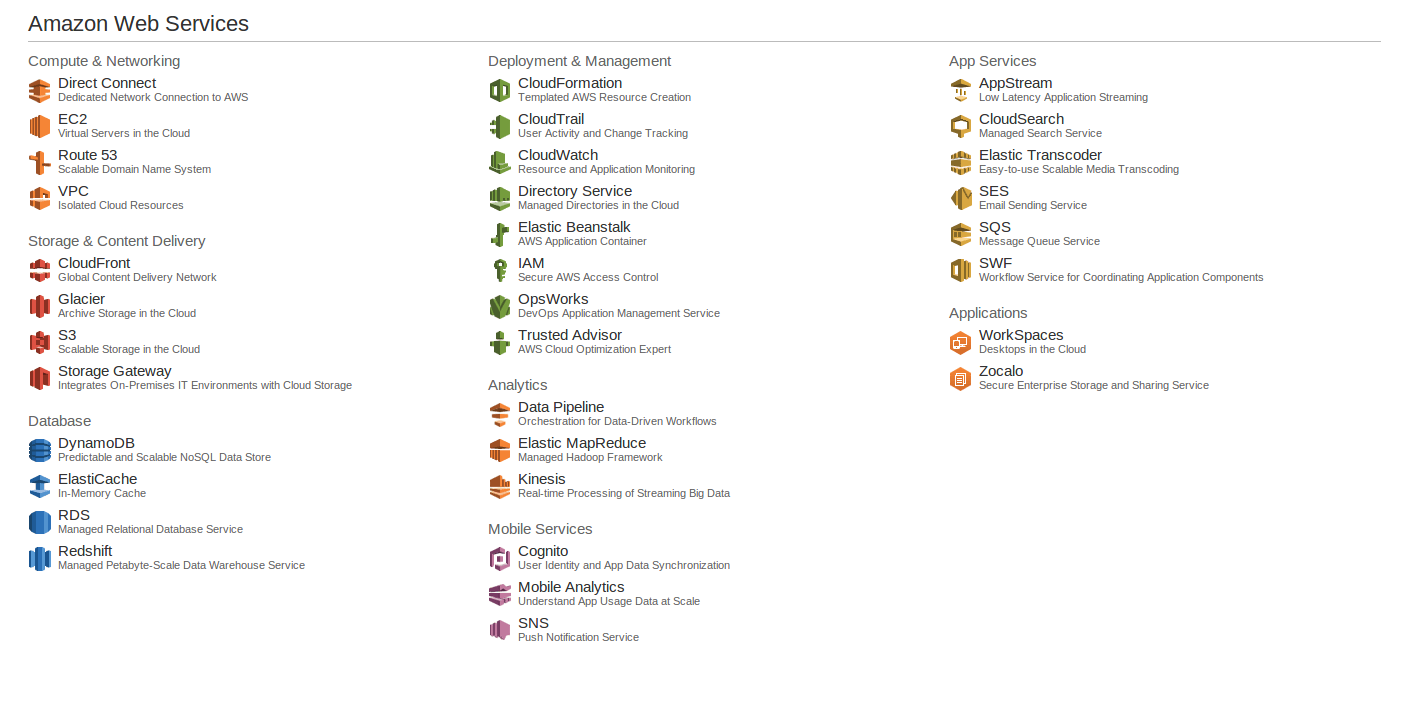
\includegraphics[width=1\textwidth]{img/aws_servicos}
    \end{center}
    \caption{Serviços da Amazon Web Services}
    \label{fig:aws_servicos}
\end{figure}

\begin{figure}[htp]
    \begin{center}
    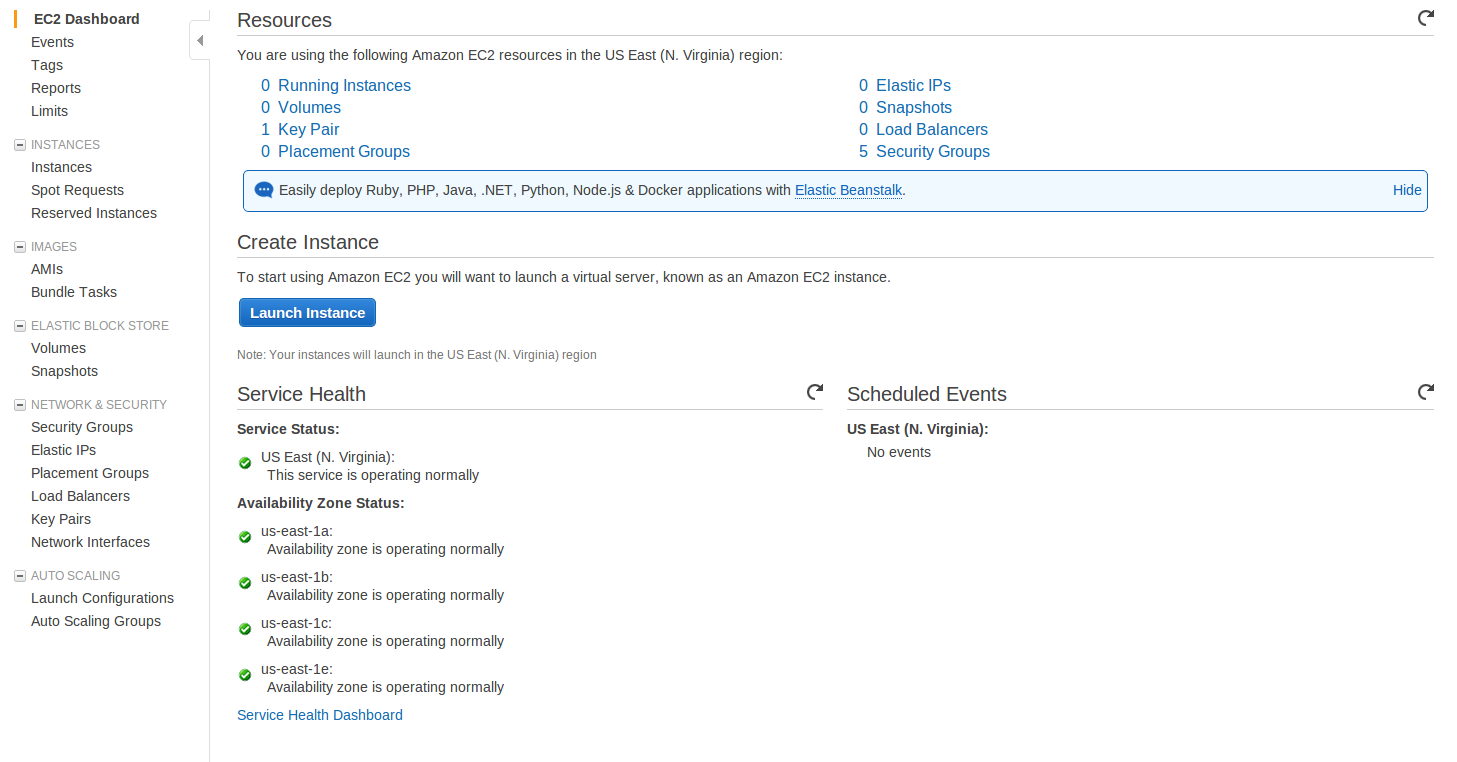
\includegraphics[width=1\textwidth]{img/aws_ec2}
    \end{center}
    \caption{Serviços de Elastic Compute Cloud (EC2)}
    \label{fig:aws_ec2}
\end{figure}

\begin{figure}[htp]
    \begin{center}
    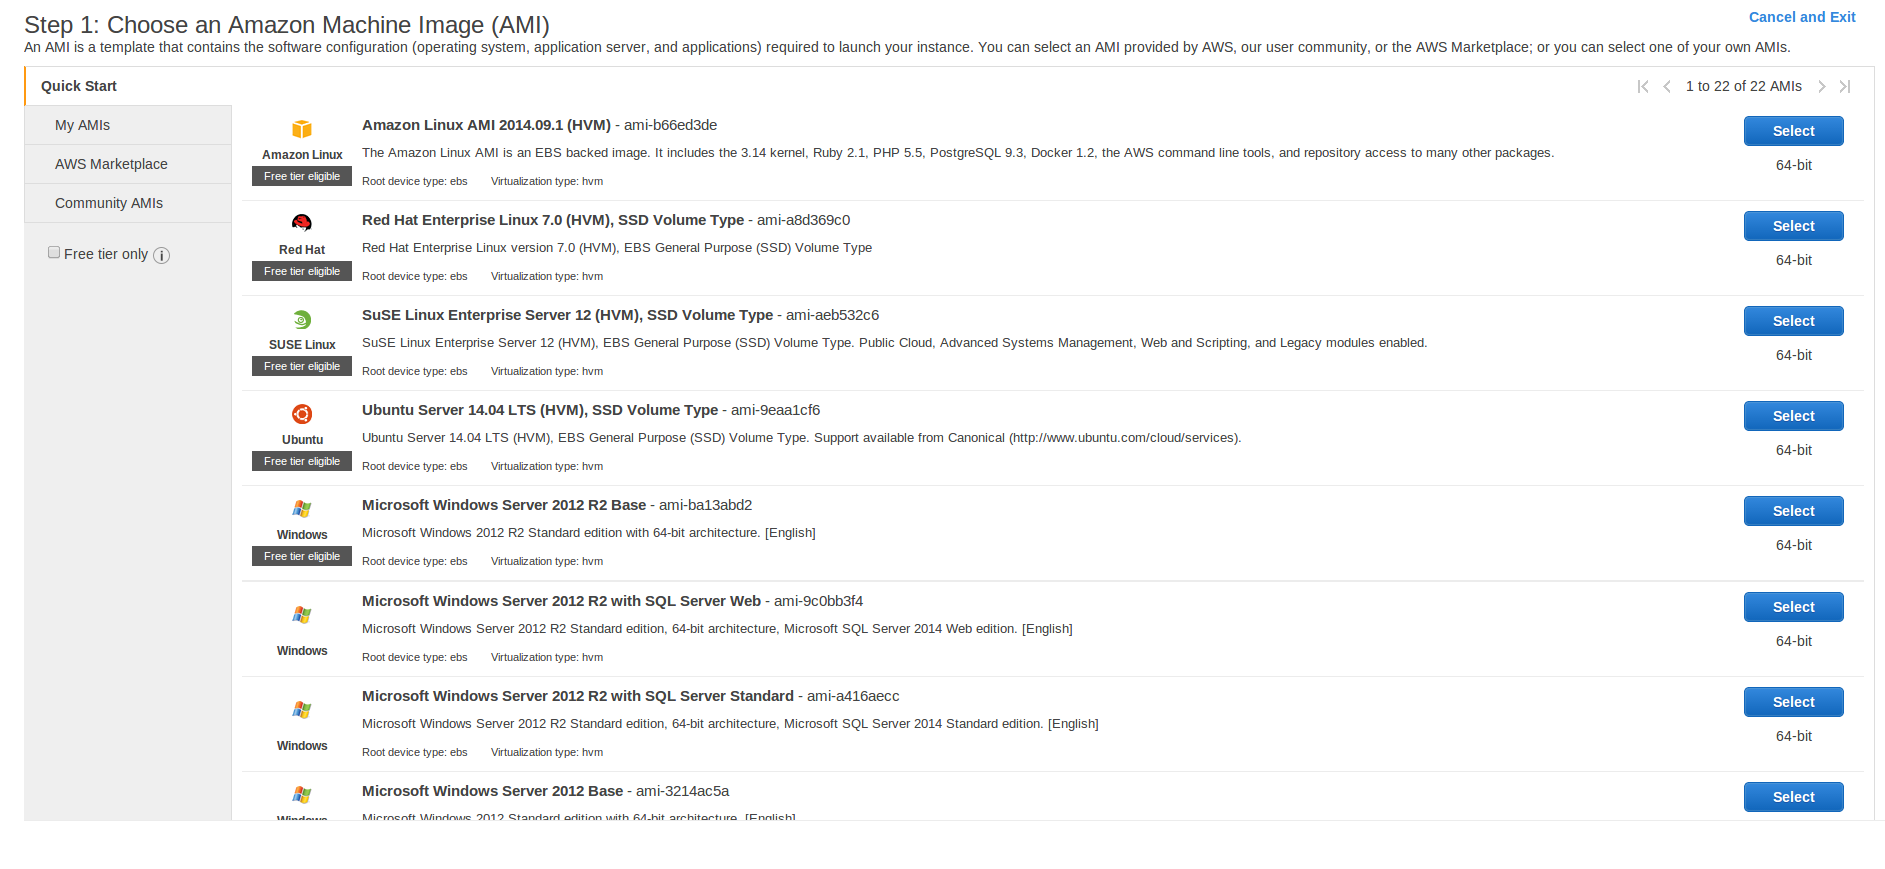
\includegraphics[width=1\textwidth]{img/aws_setup_ec2}
    \end{center}
    \caption{Escolha do tipo de configuração do software da máquina}
    \label{fig:aws_setup_ec2}
\end{figure}

\begin{figure}[htp]
    \begin{center}
    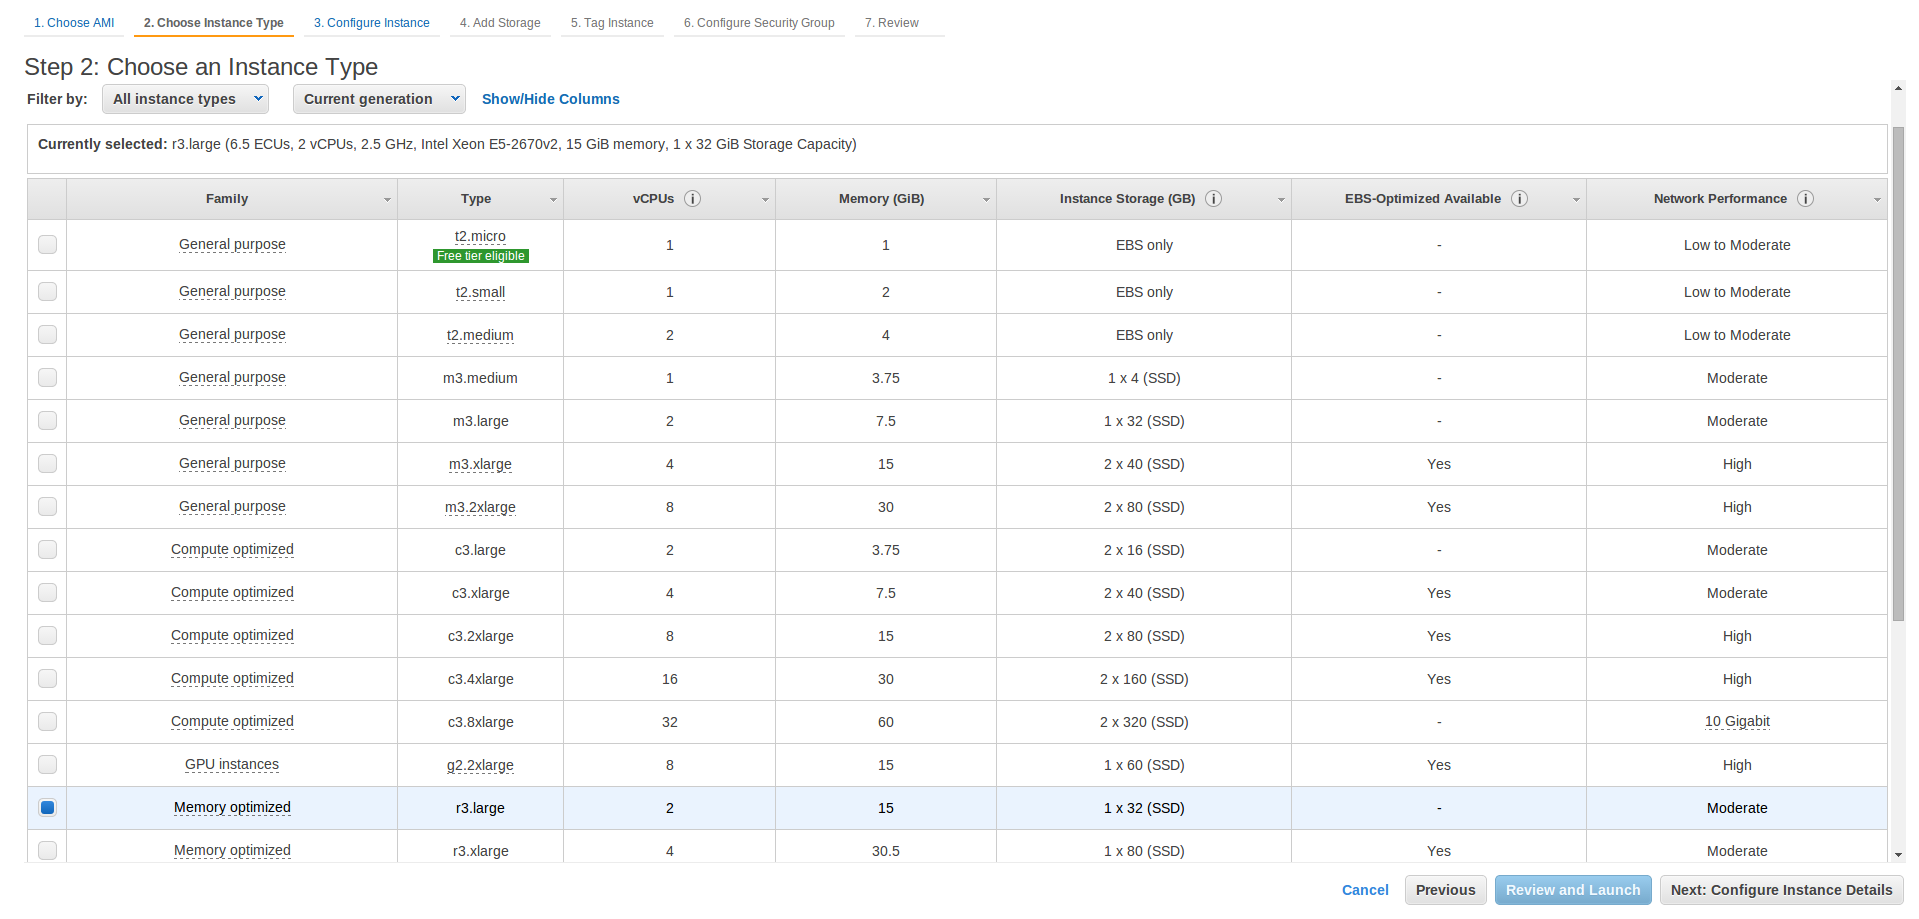
\includegraphics[width=1\textwidth]{img/aws_setup_ec2_maquina}
    \end{center}
    \caption{Escolha do tipo máquina}
    \label{fig:aws_setup_ec2_maquina}
\end{figure}

\begin{figure}[htp]
    \begin{center}
    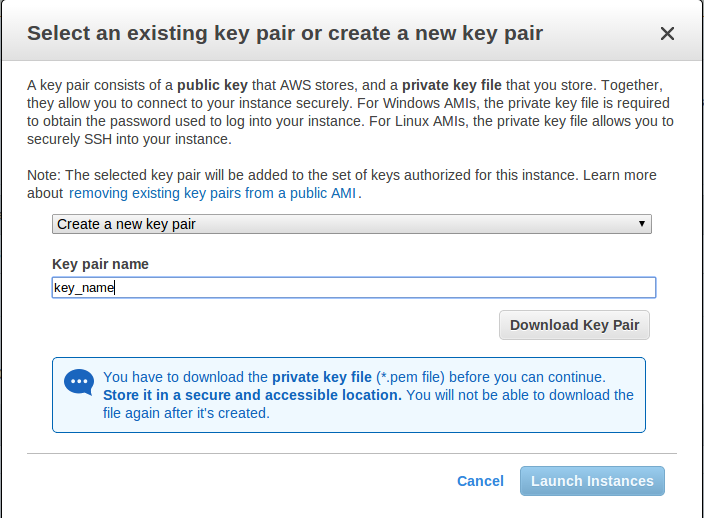
\includegraphics[width=1\textwidth]{img/aws_setup_keypair}
    \end{center}
    \caption{Criação da chave privada}
    \label{fig:aws_setup_keypair}
\end{figure}

\begin{figure}[htp]
    \begin{center}
    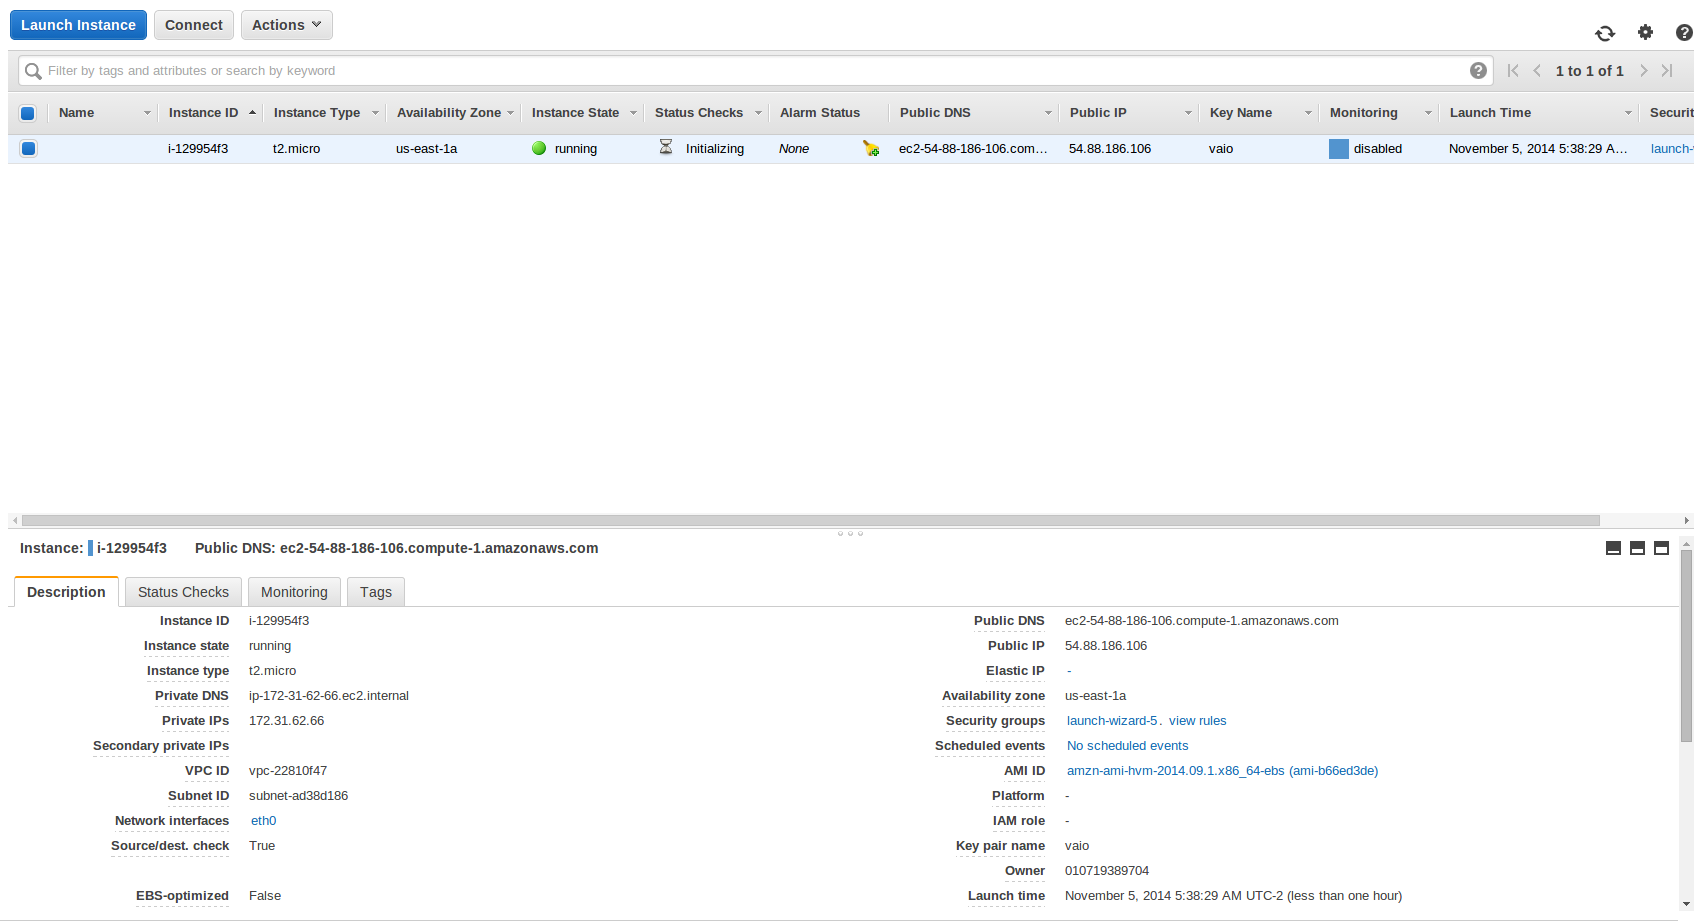
\includegraphics[width=1\textwidth]{img/aws_setup_dns}
    \end{center}
    \caption{Criação da máquina e do DNS público (Public DNS)}
    \label{fig:aws_setup_dns}
\end{figure}



Uma vez criada a máquina, deve-se utilizar a chave privada para realizar um \textit{secure shell} e se conectar remotamente ao computador

\begin{lstlisting}
ssh -i ~/Downloads/key_name.pem ec2-user@ec2-54-88-186-106.compute-1.amazonaws.com
\end{lstlisting}

Em seguida, para a automatização do ambiente de testes, criamos um arquivo \texttt{script.sh} na linguagem de programação \texttt{bash} para a rápida configuração de novas máquinas.

\begin{lstlisting}
#!/usr/bin/env bash
sudo su						# torna-se administrador. necessario para instalar pacotes no sistema operacional
yum install R				# instala o pacote R no linux
yum install git 			# instala o git para carregar os metodos de recomendacao
ssh-keygen -t rsa 		# gera a chave privada para conectar-se ao Github
cat ~/.ssh/id_rsa.pub	# depois, deve-se adicionar essa chave privada nas configuracoes do Github
git clone git@github.com:aviggiano/tcc	# clona o repositorio
cd tcc && Rscript recsys/run_tests.R 		# executa o script de avaliacao
\end{lstlisting}

